\section{Teste da Aplicação}

\subsection{Testes Unitários}

\par Os testes unitários foram realizados sobre a classe \textit{Client.java}.
Na figura abaixo pode-se ver a classe criada para os testes.\newline
Nesta classe, criaram-se as seguintes variáveis globais:
\begin{itemize}
\item 2 pontos;
\item 1 cliente;
\item 1 owner;
\end{itemize}

\par Adicionalmente criaram-se variáveis do objeto Car e Rental para verificar a correção de alguns métodos da classe visada.

\begin{figure}[H]

  \centering

  \hbox{\hspace{-6em} 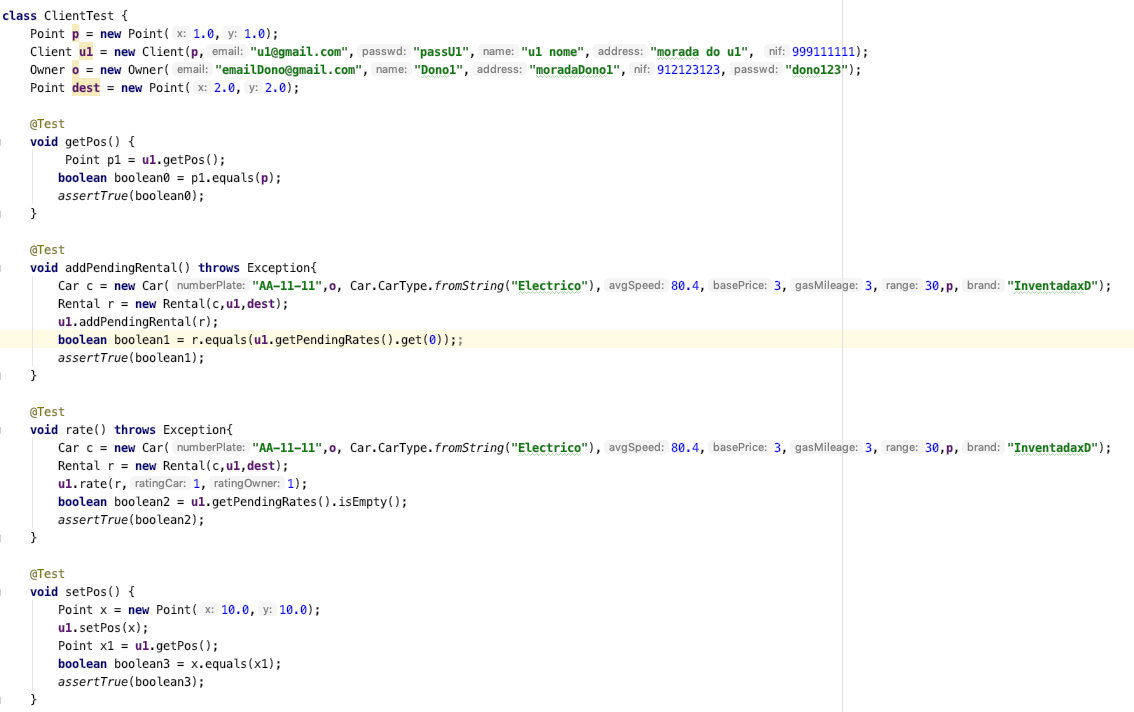
\includegraphics[scale = 0.40]{clientTest1.png}}

\end{figure}

\begin{figure}[H]

  \centering

  \hbox{\hspace{-8em} 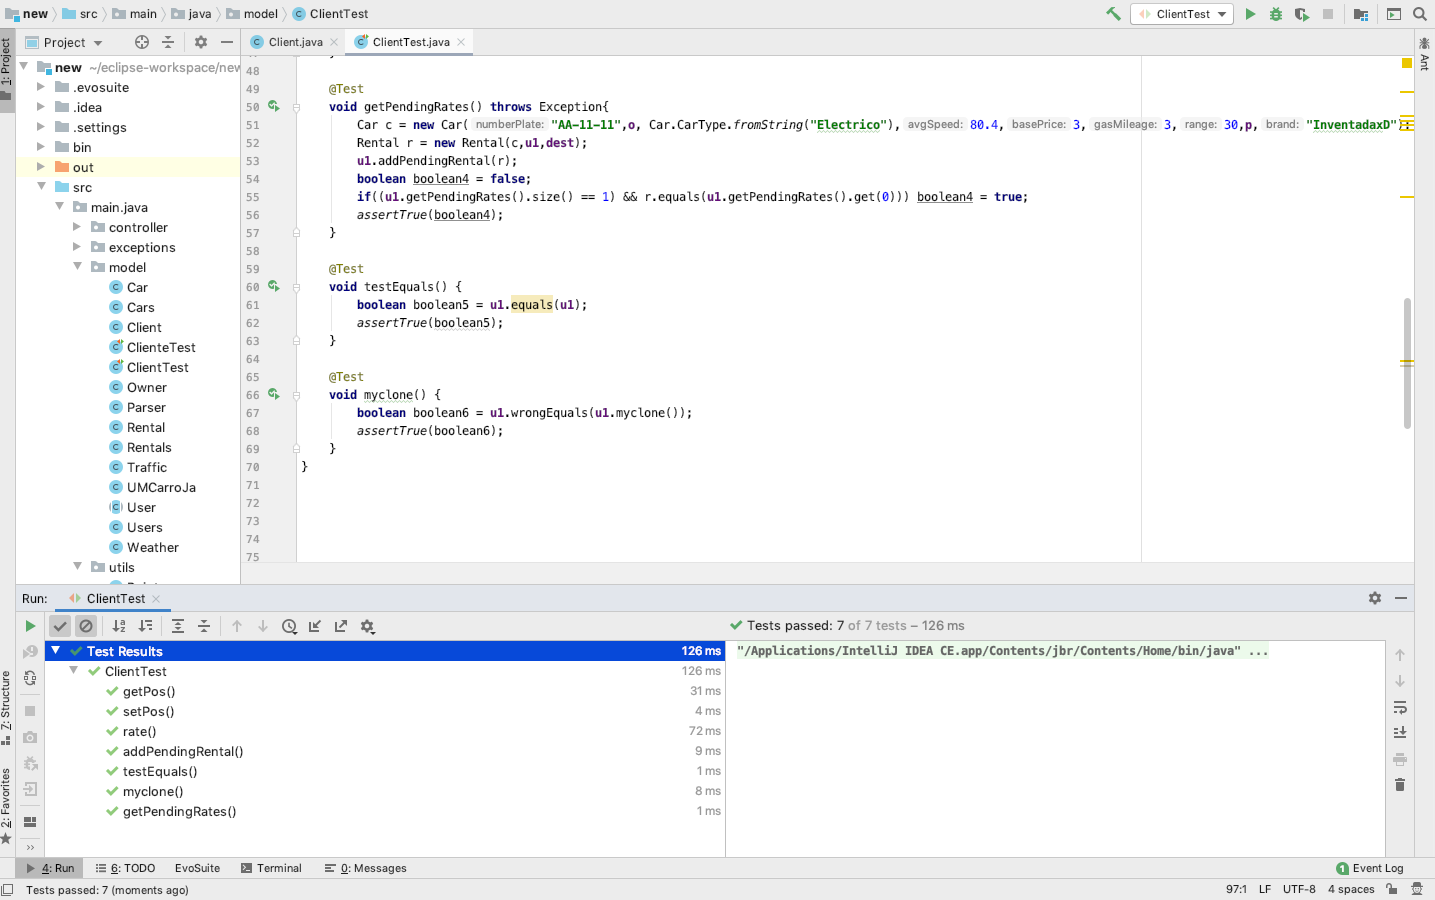
\includegraphics[scale = 0.35]{clientTestResults.png}}

  \caption {Classe ClientTest.java e resultado da sua aplicação}

  \label {fig30}

\end{figure}
\par Note-se que para testar a correção do método \textit{myclone()} foi criado um método extra na classe Cliente para verificar se os clientes partilhavam o mesmo apontador, esse método foi chamado \textit{wrongEquals()}.

\par Na figura seguinte podemos ver o código coberto por este ficheiro de testes.\newline

\begin{figure}[H]

  \centering

  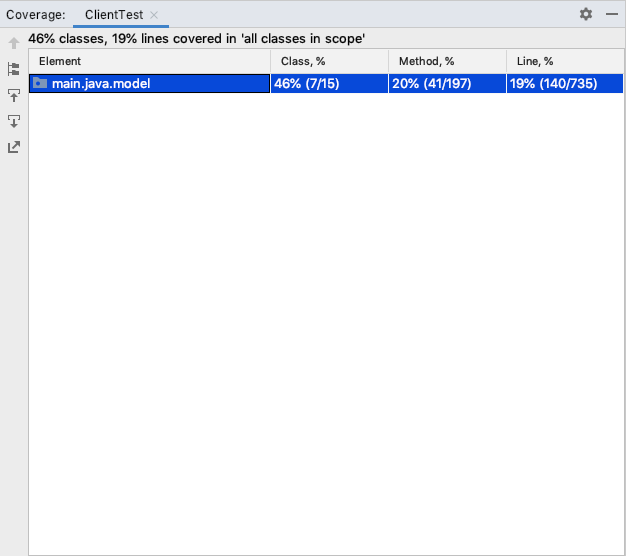
\includegraphics[scale = 0.45]{coverageClient.png}

  \caption {Cobertura da classe ClientTest.java sobre o package main.java.model}

  \label {fig31}

\end{figure}

\par \textit{Nota1:} Note-se que o facto do teste cobrir 46\% das classes do package main.java.model e 20\% dos métodos deve-se á necessidade, por parte da classe visada, de incluir objetos e recorrer a métodos de outras classes do mesmo package para ser completamente testada.\newline
\par \textit{Nota2:} Note-se que o teste de cobertura só abrange o package main.java.model. No entanto, a classe testada utiliza uma classe de nome \textit{Point.java} de outro package.

\subsection{Evosuite}

\par Para compilar o Evosuite precisei de instalar um plugin chamado Choose Runtime no InteliJ. Este foi usado para escolher a versão do JDK 1.8.0\_231 como a versão a usar para correr o Evosuite.
\par Após o Evosuite gerar os ficheiros de teste, outro problema surgiu. Os ficheiros de teste não conheciam o jUnit apesar de este estar instalado. A primeira mudança para resolver este problema foi modificar a pasta onde os testes se encontravam para que fosse reconhecida como uma pasta de test resoncs root.






















